% !TEX encoding = IsoLatin9

%%%%%%%%%%%%%%%%%%%%% SECTION 1
\section{Le perceptron}
\begin{frame}
  \begin{columns}
    \column{4.8cm}
    \tableofcontents[currentsection,hideothersubsections]
    \column{7cm}
      \centering{
      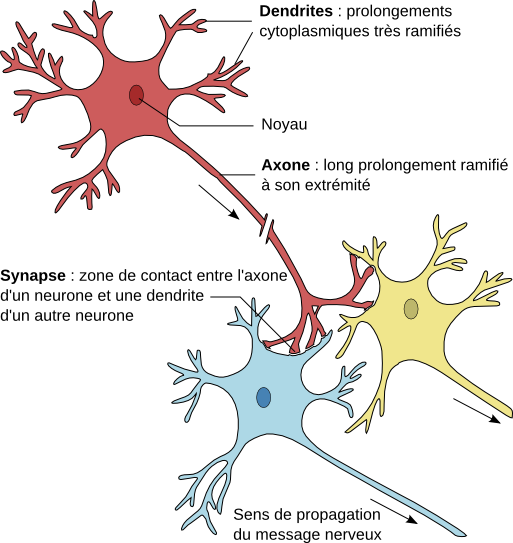
\includegraphics[width=6cm]{fig/neurone.png}
    }
  \end{columns}
  
\end{frame}


\begin{frame}
  \frametitle{Le perceptron : un neurone articiel}
  \begin{tikzpicture}[
    basic/.style={draw,fill=blue!20,text width=1em,text badly centered},
    input/.style={basic,circle},
    weights/.style={basic,rectangle},
functions/.style={basic,circle,fill=blue!10},
]
        \node[functions] (center) {};
        \node[below of=center,font=\scriptsize,text width=4em] {Fonction d'activation};
        \draw[thick] (0.5em,0.5em) -- (0,0.5em) -- (0,-0.5em) -- (-0.5em,-0.5em);
      %  \draw (0em,0.75em) -- (0em,-0.75em);
      %  \draw (0.75em,0em) -- (-0.75em,0em);
        \node[right of=center, anchor = west] (right) {$y=$ 0 ou 1};
            \path[draw,->] (center) -- (right);
        \node[functions,left=3em of center] (left) {$\sum$};
            \path[draw,->] (left) -- (center);
%        \node[weights,left=3em of left] (2) {$w_2$} -- (2) 
            \node[input,left= 4em of left] (l2) {$x_2$};
%            \path[draw,->] (l2) -- (2);
            \path[draw,->] (l2) -- node[above,midway]{$w_2$}(left);
        \node[below of=l2] (dots) {$\vdots$} ;
%(dots) node[left of=dots] (ldots) {$\vdots$};
%        \node[weights,below of=dots] (n) {$w_n$} -- (n) 
\node[input,below of=dots] (ln) {$x_n$};
%            \path[draw,->] (ln) -- (n);
            \path[draw,->] (ln) -- node[above,midway]{$w_n$}(left);
%        \node[weights,above of=2] (1) {$w_1$} -- (1) 
            \node[input,above of=l2] (l1) {$x_1$};
%            \path[draw,->] (l1) -- (1);
            \path[draw,->] (l1) -- node[above,midway]{$w_1$}(left);
%        \node[weights,above of=1] (0) {$w_0$} -- (0) 
\node[input,above of=l1] (l0) {$1$};
%            \path[draw,->] (l0) -- (0);
            \path[draw,->] (l0) -- node[above,midway]{$w_0$}(left);
        \node[below of=ln,font=\scriptsize](lin) {inputs};
        \node[right of=lin,font=\scriptsize] {weights};
    \end{tikzpicture}
\end{frame}